\documentclass[conference]{IEEEtran}

\usepackage[utf8]{inputenc}
\usepackage{cite}
\ifCLASSINFOpdf
  \usepackage[pdftex]{graphicx}
\else
  \usepackage[dvips]{graphicx}
\fi
\usepackage{amsmath}
\usepackage{array}
\usepackage{url}

% correct bad hyphenation here
% \hyphenation{op-tical net-works semi-conduc-tor}

\begin{document}
% paper title
% Titles are generally capitalized except for words such as a, an, and, as,
% at, but, by, for, in, nor, of, on, or, the, to and up, which are usually
% not capitalized unless they are the first or last word of the title.
% Linebreaks \\ can be used within to get better formatting as desired.
% Do not put math or special symbols in the title.
\title{Clean Software Architecture}

\author{\IEEEauthorblockN{Péter Ivanics}
\IEEEauthorblockA{Department of Computer Science \\
University of Helsinki \\
Email: peter.ivanics@helsinki.fi \\
\url{http://pivanics.users.cs.helsinki.fi/portfolio/}}}

\maketitle

% As a general rule, do not put math, special symbols or citations
% in the abstract
\begin{abstract}
%<Context>
The construction and the long-term maintenance of robust software architecture is a demanding task. Software architects often face the problem to ensure the extensibility of systems so that new components can be added and existing ones can be removed or replaced easily. Linearly with software growth, these aspects of software engineering are getting more and more difficult because often times the separation of concerns and the decoupling of components are not considered.  

%<Objectives>
The Clean Architecture concept was introduced recently by professional software craftsmen in order to provide principles on how to achieve robustness in software architecture engineering. This approach builds on top of the clean separation of concerns, finding the right abstractions on every level of the software projects and the minimal creation of internal dependencies.

%<Methods and objectives>
The objective of this study is to review relevant professional literature and summarize the most important aspects of Clean Architecture. The paper describes the benefits compared to other, previously suggested practices. It is explained how this approach facilitates and why is it well-suited for Object Oriented principles and software projects of the present time. 

%<Results>
Results show that understanding the key concepts, such as The Dependency Rule and the four layers of Clean Architecture, help developers to maintain robustness in their software. Ultimately, the concepts explained by this approach are independent from technologies and therefore easy to apply in every application field of our industry. 
\end{abstract}

% no keywords
% \keywords{}

\section{Introduction}
The construction and the maintenance of software is a difficult task from many aspects. Software development is a creative act of action where developers build intangible means from nothing \cite{cleancoder}. Linearly with the growth of the code base of a software project, its complexity and cost of change increases \cite{codecomplete} \cite{cleancode}, which makes developers' job even more difficult. 

Software means can be crucial for operations in industrial, business and research fields \cite{cleancode} \cite{cleancoder}. In the present time, more and more companies are established around providing software services to their customers \cite{cusumano2008changing}, and therefore software components can become business-critical assets. For this reason, the process of software development requires dedicated professionals with a lot of discipline, humility, dedication and commitment to their job \cite{cleancode}. 

Despite all the previously established standards and practices, developers often face troubles of conforming to the standards and understanding code written by them and others \cite{cleancoder}. Keeping the code base maintainable, easy to understand and open for extensions is often a challenging task \cite{cleancoder}. For this reason, the concept of Clean Code \cite{cleancode} was established which further raised the attention towards maintainable software in the industry. Agile methods and principles became popular in order to facilitate developer productivity. 

Clean Code is a concept introduced by Robert C. Martin \cite{cleancode} \cite{cleancoder}. This approach to software development brings elegant, easy to read program code in light in order to create robust, bug-free applications \cite{cleancode}. This concept is getting more and more popular among developers and even universities consider to change their approach to teach software development from the starting angle of testing and maintainable code \cite{studentscleancode}. Additionally, refactoring further increases quality of software \cite{impactofrefactoring}, which developers should not be afraid of \cite{cleancoder}. 

Software architectures establish the basis and create a good frame for quality software. During the last decades, many different approaches and design patterns were developed and proposed by professionals to facilitate robustness of programs \cite{codecomplete} \cite{onionarchitecture} \cite{gof}, which are widely used and appreciated by other developers worldwide. In order to ensure maintainable and robust software systems, a loosely coupled, flexible and extensible frame should be provided as the basis. 

For this reason, an approach to Clean Architecture is emerging \cite{cleanarchitecture} building on top of Clean Code principles. This paper aims to seek answers to the following research questions by discussing relevant literature in the topic: 

\begin{enumerate}
	\item what are the main aspects of the Clean principles in terms of software architecture?
	\item why such architecture is needed, why it can be meaningful for any software project independently from technology and platform?
\end{enumerate}  

The rest of this paper is structured, as follows. The next section introduces... Chapter III focuses on...
 Chapter IV discusses... Finally, the last chapter concludes the findings of this research and establishes the directions for any further research. 
%TODO

\section{The need for a clean design}
Software development is collaborative work. More and more developers work in teams of various size on multiple technologies to develop their software day-by-day. Inevitably, components are getting bigger and are developed simultaneously by multiple coders. Linearly as time passes, developers tend to have difficulties understanding the code they have written, because they do not remember what the intention behind the lines were \cite{cleancoder}. Similarly, understanding decisions made and code written by fellow colleagues is even more difficult and challenging on every level of abstraction \cite{cleancoder}. As the code base grows, decisions that were previously made may need to be reconsidered and code may need to be refactored to enhance its reliability. 

For this reason, considering the intent behind a decision is key even on the lowest level of components, for instance classes, objects, functions or even variable names. The usage of intention-revealing names on all parts of software projects greatly enhance the readability of their code \cite{cleancode}. This enables developers to read and understand others' code more efficiently and work on code written by others with more confidence. 

Demonstrating the intent behind design decisions is a key characteristic of good design which helps developers to understand what the program code does. This is particularly important while debugging or refactoring detailed parts of the code. However, it is not limited to low-level components of the software. A well-designed system-wide architecture shares the same, meaningful separation of concerns \cite{cleancode} \cite{cleanarchitecture} \cite{onionarchitecture}. By separating responsibilities in the application, the code not only gets easier to understand but also more flexible, loosely coupled and easier to test \cite{cleancoder}. 

Consequently, to allow understanding the software architecture on its highest level, clear decisions should be made on the responsibility of the components. Once the components are chosen, their name should tell right away the intent they were made for. Applying the same approach on every level of abstracting throughout the application is crucial as it usually gives a good direction for the development.

\section{Principles}
Communicating the intent behind the components is a good start for a Clean Architecture. Nevertheless, there are some other principles which help developers to avoid tight coupling and complex connections between the objects. The aim should be an approach, where each component is standalone and are handled as plugins to other components \cite{cleancode} \cite{cleanarchitecture}. In other words, components should be independent, which leads to the first principle of Clean Architecture, namely, the Dependency Rule \cite{cleanarchitecture}. 

\subsection{The Dependency Rule}
The Dependency Rule dictates, that the lower level components, such as database, 

\begin{figure}[!t]
\centering
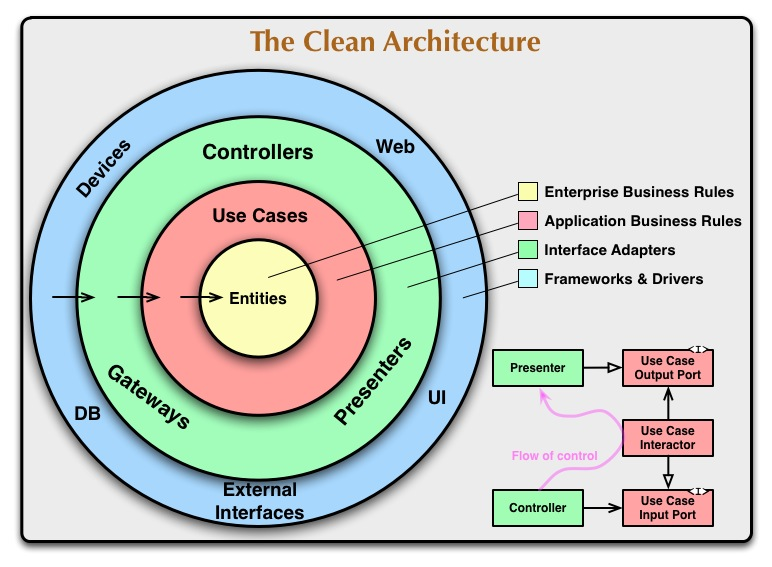
\includegraphics[width=3in]{images/cleanarchitecture.jpg}
\caption{The Clean Architecture \cite{cleanarchitecture}.}
\label{fig_sim}
\end{figure}

\subsection{Testability}

\subsection{Separation of concerns}

% An example of a floating figure using the graphicx package.
% Note that \label must occur AFTER (or within) \caption.
% For figures, \caption should occur after the \includegraphics.
% Note that IEEEtran v1.7 and later has special internal code that
% is designed to preserve the operation of \label within \caption
% even when the captionsoff option is in effect. However, because
% of issues like this, it may be the safest practice to put all your
% \label just after \caption rather than within \caption{}.
%
% Reminder: the "draftcls" or "draftclsnofoot", not "draft", class
% option should be used if it is desired that the figures are to be
% displayed while in draft mode.
%
%\begin{figure}[!t]
%\centering
%\includegraphics[width=2.5in]{myfigure}
% where an .eps filename suffix will be assumed under latex, 
% and a .pdf suffix will be assumed for pdflatex; or what has been declared
% via \DeclareGraphicsExtensions.
%\caption{Simulation results for the network.}
%\label{fig_sim}
%\end{figure}

% Note that the IEEE typically puts floats only at the top, even when this
% results in a large percentage of a column being occupied by floats.


% An example of a double column floating figure using two subfigures.
% (The subfig.sty package must be loaded for this to work.)
% The subfigure \label commands are set within each subfloat command,
% and the \label for the overall figure must come after \caption.
% \hfil is used as a separator to get equal spacing.
% Watch out that the combined width of all the subfigures on a 
% line do not exceed the text width or a line break will occur.
%
%\begin{figure*}[!t]
%\centering
%\subfloat[Case I]{\includegraphics[width=2.5in]{box}%
%\label{fig_first_case}}
%\hfil
%\subfloat[Case II]{\includegraphics[width=2.5in]{box}%
%\label{fig_second_case}}
%\caption{Simulation results for the network.}
%\label{fig_sim}
%\end{figure*}
%
% Note that often IEEE papers with subfigures do not employ subfigure
% captions (using the optional argument to \subfloat[]), but instead will
% reference/describe all of them (a), (b), etc., within the main caption.
% Be aware that for subfig.sty to generate the (a), (b), etc., subfigure
% labels, the optional argument to \subfloat must be present. If a
% subcaption is not desired, just leave its contents blank,
% e.g., \subfloat[].


% An example of a floating table. Note that, for IEEE style tables, the
% \caption command should come BEFORE the table and, given that table
% captions serve much like titles, are usually capitalized except for words
% such as a, an, and, as, at, but, by, for, in, nor, of, on, or, the, to
% and up, which are usually not capitalized unless they are the first or
% last word of the caption. Table text will default to \footnotesize as
% the IEEE normally uses this smaller font for tables.
% The \label must come after \caption as always.
%
%\begin{table}[!t]
%% increase table row spacing, adjust to taste
%\renewcommand{\arraystretch}{1.3}
% if using array.sty, it might be a good idea to tweak the value of
% \extrarowheight as needed to properly center the text within the cells
%\caption{An Example of a Table}
%\label{table_example}
%\centering
%% Some packages, such as MDW tools, offer better commands for making tables
%% than the plain LaTeX2e tabular which is used here.
%\begin{tabular}{|c||c|}
%\hline
%One & Two\\
%\hline
%Three & Four\\
%\hline
%\end{tabular}
%\end{table}

\section{Conclusion}
The conclusion goes here.

\begin{thebibliography}{1}

  \bibitem{cleanarchitecture}
R. C. Martin. (2012, Aug. 13) \emph{The Clean Architecture} [Online]. Available: \url{https://8thlight.com/blog/uncle-bob/2012/08/13/the-clean-architecture.html}

\bibitem{cleancoder}
R. C. Martin. \emph{The Clean Coder: A Code of Conduct for Professional Programmers}, 1st ed. Boston, MA, Pearson Education, Inc. 2011. 

\bibitem{cleancode}
R. C. Martin. \emph{Clean Code: A Handbook of Agile Software Craftsmanship}, 1st ed. Boston, MA, Pearson Education, Inc. 2008.

\bibitem{onionarchitecture}
J. Palermo. \emph{The Onion Architecture} [Online]. Available: \url{http://jeffreypalermo.com/blog/the-onion-architecture-part-1/}

\bibitem{codecomplete}
S. Steve McConnell. \emph{Code Complete: A Practical Handbook of Software Construction}, 2nd ed. Microsoft Press. 2004.

\bibitem{cusumano2008changing}
M. Cusumano. \emph{The Changing Software Business: From Products to Services and Other New Business Models Paper 236}. MIT Center for Digital Business. 2007.

\bibitem{gof}
E. Gamma, R. Helm, R. Johnson, J. Vlissides \emph{Design Patterns: Elements of Reusable Object-Oriented Software}, 1st ed. Addison Wesley. 1994.

\bibitem{impactofrefactoring}
M. Wahler, U. Drofenik, W. Snipes. \emph{Improving Code Maintainability: A Case Study on the Impact of Refactoring}. 2016 IEEE International Conference on Software Maintenance and Evolution. 2016.

\bibitem{studentscleancode}
M. Doyle, B. Buckley, W. Hao,  J. Walden. \emph{Work in Progress - Does Maintenance First Improve Student's Understanding and Appreciation of Clean Code and Documentation}. Frontiers in Education Conference (FIE). 2011.
% http://hillside.net/patterns

% Swift Design Patterns: The Easy Way; Standard Solutions for Everyday Programming Problems; Great for: Game Programming, System Analysis, App Programming, ... & Database Systems (Design Patterns Series) https://www.amazon.com/Swift-Design-Patterns-Solutions-Programming-ebook/dp/B01N2KE1T7/ref=sr_1_8?ie=UTF8&qid=1488874232&sr=8-8&keywords=software+patterns

\end{thebibliography}
\end{document}
